\documentclass{article}
\usepackage[utf8]{inputenc}
\usepackage[margin=1.2in]{geometry} % smaller margins please

\title{Programmering 2 eksamensnoter}
\author{
  Andreas Troelsen\\
  \texttt{andtro87@cs.au.dk}
  \and
  Mathias Bak Bertelsen\\
  \texttt{bufas@cs.au.dk}\\
%  \texttt{http://mathiasbak.dk}
}
\date{December 24, 2012}

\usepackage{natbib}
\usepackage{graphicx}

\usepackage{amsmath}  % For math stuff
\usepackage{qtree}    % For tree-structures (recursion.tex)
\usepackage{tikz}

\begin{document}

%\tikzstyle{block} = [draw, fill=blue!20, rectangle, 
    minimum height=3em, minimum width=6em]
\tikzstyle{sum} = [draw, fill=blue!20, circle, node distance=1cm]
\tikzstyle{input} = [coordinate]
\tikzstyle{output} = [coordinate]
\tikzstyle{pinstyle} = [pin edge={to-,thin,black}]

% The block diagram code is probably more verbose than necessary
\begin{tikzpicture}[auto, node distance=2cm,>=latex']
    % We start by placing the blocks
    \node [input, name=input] {};
    \node [sum, right of=input] (sum) {};
    \node [block, right of=sum] (controller) {Controller};
    \node [block, right of=controller, pin={[pinstyle]above:Disturbances},
            node distance=3cm] (system) {System};
    % We draw an edge between the controller and system block to 
    % calculate the coordinate u. We need it to place the measurement block. 
    \draw [->] (controller) -- node[name=u] {$u$} (system);
    \node [output, right of=system] (output) {};
    \node [block, below of=u] (measurements) {Measurements};

    % Once the nodes are placed, connecting them is easy. 
    \draw [draw,->] (input) -- node {$r$} (sum);
    \draw [->] (sum) -- node {$e$} (controller);
    \draw [->] (system) -- node [name=y] {$y$}(output);
    \draw [->] (y) |- (measurements);
    \draw [->] (measurements) -| node[pos=0.99] {$-$} 
        node [near end] {$y_m$} (sum);
\end{tikzpicture}



\maketitle
\tableofcontents
\newpage

\subsection{Læs dette først!}

Dokumentet er ment som en hjælp til at læse op til Programmering 2 eksamen. Det er på ingen måde komplet, og vi giver ingen garanti for korrektheden af indholdet. Hvis du opdager fejl, eller har forslag til forbedringer, er du mere end velkommen til at skrive til en af os. Emails findes på forsiden af dokumentet.

Dokumentet er opbygget på den måde at det er et kapitel for hvert eksamensemne. Først er der noter til emnet og til sidst to eksempler på dispositioner. Nogle af punkterne i dispositionerne er markeret med fed skrift - det er disse punkter, vi anbefaler, at du skriver på tavlen, efter du har trukket dit emne.

\subsection{Generelt om mundtlig eksamen}
Det er vigtigt at forberede sig godt på emnerne og komme i gang i god tid. Det tager som regel længere tid at forberede sig, end man regner med. En god teknik er at arbejde sammen i grupper af to eller tre personer og fremlægge for hinanden. På denne måde får man feedback med det samme og kan således nå at forbedre sin fremlæggelse inden eksamen. Tag også tid på dine fremlæggelser. Det er vigtigt at tiden passer nogenlunde, så du får sagt alt det, du gerne vil, og at du ikke er færdig efter fem minutter. "Øvelse, øvelse, øvelse... og atter øvelse" - Holger A. Nielsen.

Det kan derudover være en god ide at overvære hinandens eksamener. Aftal med din læsemakker, at I går med ind til hinandens eksamener. På den måde kan I få ekstra feedback på jeres præsentation, og dermed forbedre jer til næste eksamen. Husk på, at skulderklap ikke hjælper ret meget, så man skal kunne tåle at høre, hvad man har gjort galt. Udover at få god feedback finder du også ud af, hvilke spørgsmål censor og eksaminator stiller, og muligvis hvilke emner, der bør undgås.

\subsection{Fremlæggelse af patterns}
Når du skal fremlægge et pattern er det vigtigt at have styr på tre ting:
\begin{itemize}
    \item UML diagrammet for det pågældende pattern skal være helt på plads. Pilene skal tegnes korrekt og der skal være styr på relationerne mellem klasser og interfaces. Det kan være en god ide at tegne dette som noget af det første, da du resten af tiden vil kunne referere til det og kigge på det, hvis du glemmer noget.
    \item Hilvket problem dette pattern løser og i hvilke situationer det er relevant at benytte. Dette er skrevet på punktform for hvert pattern i Horstmann-bogen, så det burde ikke være så svært at finde ud af.
    \item Et konkret ksempel på brug. Sørg for at have et godt eksempel som du føler dig tryg ved (brug fx afleveringerne, hvis det specifikke pattern er blevet anvendt i en aflevering). Hvis du ikke selv bringer det op kan du risikere at blive spurgt. Det kan være svært at finde på et godt eksempel midt under eksaminationen.
\end{itemize}


% RECURSION
\section{Recursive Methods \& Data Structures}

Rekursive metoder er metoder, som kalder sig selv. Rekursion kan i nogle tilfælde gøre kodestykker meget kortere og være meget lettere at implementere end iteration (fx Koch-kurver). Derimod kan rekursion nemt være meget langsommere, og nogle gange fylde meget mere i hukommelsen, hvis man ikke er varsom.

\subsection{Fibonacci}

\begin{itemize}
  \item Fibonacci-tallene er et godt eksempel på en noget som kan defineres som en rekursiv funktion. Sekvensens definition siger, at hvert nyt tal i sekvensen er summen af de to foregående tal, og de to første tal er begge 1. Kvadrater med sidelængde af disse tal kan sættes op omkring hinanden i spiraler. 
  \begin{itemize}
    \item Sekvensen ser således ud: 1, 1, 2, 3, 5, 8, 13, 21, 34, etc.
    \item $1+1=2$, $2+1=3$, $3+2=5$, $5+3=8$, etc.
  \end{itemize}

  \item Rekursivt kan metoden defineres således:
  \[
    F_n =
    \begin{cases}
      1                 & n \in \{1,0\} \\
      F_{n-1} + F_{n-2} & n > 1
    \end{cases}
  \]
  \item Man kan skrive en tilsvarende metode i Java således:
  \begin{itemize}
    \item
      \begin{verbatim}
    public int fib(int n) {
        if (n == 0 || n == 1)
            return 1;
        return fib(n-1) + fib(n-2);
    }
      \end{verbatim}
    \item Testen for om n er 0 eller 1 kaldes en stopbetingelse. En rekursiv metode bør altid have en stopbetingelse, så man er sikker på, at den ikke fortsætter med at kalde sig selv uendeligt.
  \end{itemize}

  \item Rekursive kald giver anledning til visualisering vha. træstrukturer. For et kald til fib(4) laves to yderligere kald, fib(3) og fib(2), og hver af disse kald laver yderligere to kald, etc. Følgende træstruktur viser kaldet til fib(4):

  \Tree [.fib(4)  [.fib(3)
                      [.fib(2) 
                          [.fib(1) ]
                          [.fib(0) ] ]
                      [.fib(1) ] ]
                  [.fib(2) 
                      [.fib(1) ]
                      [.fib(0) ] ] ]
  \item Bemærk, at fib(2) og fib(0) kaldes to gange, mens fib(1) kaldes tre gange. Dette er et perfekt eksempel på en langsom/ineffektiv implementation, hvor de samme værdier beregnes flere gange.
\end{itemize}

\subsection{Fraktaler}

\begin{itemize}
  \item Fraktaler er rekursiv grafik. Fraktaler er kurver som aldrig er glat nok til at kunne approximeres med linjestykker. Hvis man “zoomer ind” på en fraktal vil den altid “udfolde sig” mere. Velkendte fraktaler inkluderer Mandelbrot-mængden, Sierpinski-trekanter og Koch-linjer.
  \begin{itemize}
    \item En Koch-linje er et linjestykke med et “trekantet hak” i midten, som gør at hvert linjestykke brydes ned i fire linjestykker, som hver brydes ned i fire linjestykker, osv.
    
    \begin{center}
      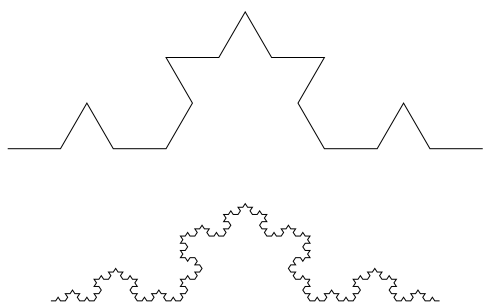
\includegraphics[scale=0.7]{images/koch_line.png}
    \end{center}
    
    \item Koch-linjen kan defineres rekursivt vha. et “tegneobjekt”, fx et Crayon objekt $c$, hvis \verb|turn(x)| metode drejer objektet $x$ grader, og \verb|move(y)| tegner en streg af længde $y$.
    \begin{verbatim}
      private void kochLine(int order, double len) {
          // Stopkriterie
          if (order == 0) c.move(len);
        
          // Rekursionsskridt
          kochLine(order-1,len/3); c.turn(-60);
          kochLine(order-1,len/3); c.turn(120);
          kochLine(order-1,len/3); c.turn(-60);
          kochLine(order-1,len/3);
      }
    \end{verbatim}
    \item Hvis stopbetingelsen ikke er opfyldt vil hvert kald til kochLine lave 4 rekursive kald. Det bliver derfor meget hurtigt kompliceret manuelt at gennemløbe sådan en metode, og træstrukturen vil blive meget bred, meget hurtigt.
  \end{itemize}
\end{itemize}

\subsection{Evaluering af udtryk}

\begin{itemize}
  \item Rekursion kan bruges til evaluering af matematiske udtryk. Man kan have et udtryk som $3+4*5$, som ikke beregnes “lineært”. Her kan man opdele de matematiske udtryk i forskellige elementer.
  \begin{itemize}
    \item Operatorer
    \item Deludtryk, som kan være enten et tal eller endnu et deludtryk
    
    \begin{center}
      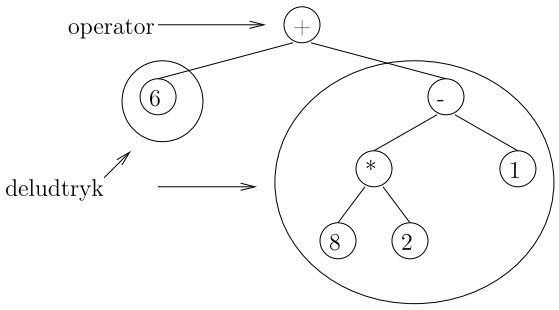
\includegraphics[scale=0.7]{images/syntax_tree_math.png}
    \end{center}
    
  \end{itemize}
  
  \item På den måde vil en metode, fx \verb|getValue(String exp)| kalde sig selv rekursivt, hver gang den har brudt et udtryk ned i to deludtryk. Når deludtrykkene til sidst udmunder i tal bliver der langsomt returneret delværdier, indtil hele udtrykket er beregnet.
  
    \begin{center}
      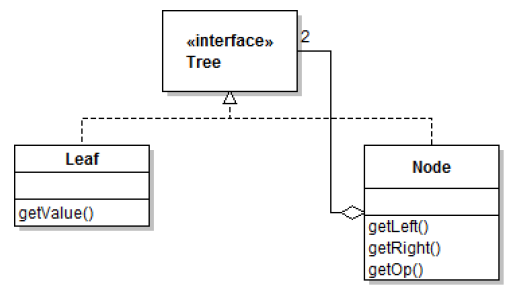
\includegraphics[scale=0.8]{images/composite_pattern.png}
    \end{center}
  
\end{itemize}


\subsection{Dispositionsforslag 1}

\begin{itemize}
    \item \textbf{Hvad er rekursion?}
    \begin{itemize}
        \item Fordele: simplere kode, let at implementere
        \item Ulemper: adskillige 'pitfalls'
    \end{itemize}
    
    \item \textbf{Rekursive metoder}
    \begin{itemize}
        \item Fibonacci-tal
        \item Rekursionstræer
    \end{itemize}
    
    \item \textbf{Rekursive datastrukturer}
    \begin{itemize}
        \item Tree, Node, Leaf
        \item UML-diagram
    \end{itemize}
    
    \item \textbf{Visitor Pattern}
    \begin{itemize}
        \item UML-diagram
        \item accept(), visitNode() og visitLeaf()
        \item FileSystemNode-aflevering
        \item Sammenlign med Composite Pattern
    \end{itemize}
    
\end{itemize}

\subsection{Dispositionsforslag 2}

\begin{itemize}
    \item \textbf{Rekursion vs iteration}
    \begin{itemize}
        \item Stopkriterie og rekursionstilfælde (skriv matematisk notation og kode for fibonacci eller fakultet)
        \item Mange problemer er rekursive af natur og derfor simplere at løse på denne måde. Kodens læsbarhed kan også øges markant.
        \item Eks. nyttigt til fraktaler (husk dIntProg)
        \item Kan være (meget!) ineffektivt i forhold til iteration (kan føre til stackoverflow)
        \item Tegn kald-træ for fibonacci
        \item Tradeoff mellem simplicitet og effektivitet
    \end{itemize}

    \item \textbf{Visitor pattern}
    \begin{itemize}
        \item Referer til afleveringen
        \item Tegn UML og forklar hvordan et accept()-kald fungerer
        \item \textbf{Composite pattern}
    \end{itemize}
\end{itemize}

% CLASS DESIGN
\section{Class Design \& Invariants}

En klasse er en samling af fields og metoder. Ofte bruges klasser som skabeloner, som objekter kan instantieres fra. Nogle klasser kan således betragtes som "blueprints", som man kan skabe objekter ud fra. Et velgennemtænkt og godt struktureret klassedesign er meget vigtigt for brugbarhed af klasser.

\subsection{Klassestruktur}

\begin{itemize}
  \item Klasser indeholder typisk nogle fields, en eller flere constructors og en række metoder. Klassens fields udgør dens tilstand, og dens metoder udgør dens interface (klasse-interface).
  \item Constructors sørger for at objekter instantieres fra klasser med nogle bestemte værdier for deres fields, dvs. en starttilstand.
  \item Metoder er "funktioner" som kan kaldes på klassen selv (static), eller på individuelle objekter instantieret fra en klasse
  \item Utility-klasse: En klasse med en private constructor (kan ikke instantieres), og udelukkende static metoder (fx Math, Collections).
\end{itemize}

\subsection{Indkapsling}

\begin{itemize}
  \item Visibility modifiers: public/private/protected
  \begin{itemize}
    \item Constructors er generelt public.
    \item Metoder kan være begge dele. Ofte bruges private metoder som hjælpemetoder til public metoder. (Én gang public, altid public - gælder også for protected)
    \item Fields bør altid være private, og objekters/klassers tilstande bør altid tilgås/manipuleres gennem public metoder.
  \end{itemize}
  
  \item static
  \begin{itemize}
    \item Fields og metoder tagged som static er tilgængelige på klassen selv, og alle objekter instantieret fra klassen. Static fields deles mellem alle objekter af klassen.
    \item Static metoder (kaldes på klassen) kan kun tilgå static fields.
    \item Non-static metoder (kaldes på objekter) kan tilgå både static og non-static fields.
  \end{itemize}
  
  \item Et objekts tilstand (dvs. fields) aflæses gennem "accessorer" (fx \verb|get()| metoder), og modificeres gennem "mutatorer" (fx \verb|set()| metoder).
  \begin{itemize}
    \item Objekters tilstande må aldrig modificeres af accessorer (da de så vil være mutatorer), men de må gerne aflæses af mutatorer, så længe der samtidig er en tilsvarende accessor-metode, som aflæser tilstandene uden at ændre på dem.
    \item Scanner er et godt eksempel på dårlig stil: Ingen accessor (\verb|getCurrent()|), så hvis man skal bruge det “nuværende” element skal man efter kaldet til \verb|next()| gemme værdien/referencen i en lokal variabel, da \verb|next()| flytter cursoren ét element frem inden den returnerer et element.
  \end{itemize}
  
  \item Et objekt er mutérbart, hvis dets fields kan manipuleres med enten via direkte adgang (public) eller gennem mutator-metoder. Omvendt kaldes det immutérbart, hvis det kun består af accessor-metoder (fx String), og således ikke kan ændres på, efter det er blevet skabt.
  \begin{itemize}
    \item Kun immutérbare objekter bør deles mellem andre objekter.
    \item Mutérbare objekters indre tilstand kan ændres, hvis deres fields af reference-typer returneres direkte af \verb|get()| metoder (fx ArrayList, HashMap), da sådanne return-values returnerer objekt-referencen, fremfor blot at returnere en simpel værdi (som med primitive typer).
    \item Hvis mutérbare objekter skal returneres i \verb|get()| metoder bør objekterne klones først vha. \verb|clone()|.
    \item På samme måde bør constructors klone eventuelle mutérbare objekter, som de får som parametre.
  \end{itemize}
\end{itemize}

\subsection{Cloning}

\begin{itemize}
  \item Deep/shallow clone.
\end{itemize}
  
\subsection{Quality of class interfaces}

\begin{itemize}
  \item Cohesion: En klasse er "cohesive" eller sammenhængende, hvis dens metoder alle har at gøre med det samme overordnede emne. Fx en Mailbox-klasse som kun har metoder, som har at gøre med breve/beskeder.
  \item Completeness: En klasse er "complete" eller fuldstændig, hvis den har metoder til ethvert tænkeligt formål indenfor dens scope. Fx Math-klassen, som har en stor mængde metoder til matematiske beregninger (dog ingen metoder til beregning af egentlige brøker, dvs. ikke helt complete).
  \item Convenience: En klasse er "convenient" eller bekvem, hvis simple operationer og opgaver er nemme at løse. Et klasseinterface skal være nemt at bruge, så brugere ikke skal kalde 10 forskellige metoder for at få et simpelt resultat.
  \item Clarity: En klasse er "clear" eller letforståelig, når der ikke kan opstå meget forvirring omkring dens interface. ListIterator's \verb|next()| og \verb|add()| metoder er meget analog til hvordan et tekstbehandlingsprogram virker, men dens \verb|remove()| metode er meget klodset. Dårlig clarity.
  \item Consistency: En klasse er "consistent" hvis dens metoder ikke afviger i fx parameter-syntax. Fx tager Java's GregorianCalendar klasse et månednummer mellem 0 og 11, men et dagnummer mellem 1 og 31, i dens constructor, hvilket er meget fjollet.
\end{itemize}

\subsection{Programming by contract}

\begin{itemize}
  \item En måde at undgå tunge, performance-sænkende gyldighedschecks. Ved at opstille "kontrakter" for hvordan metoder må/skal benyttes kan man fralægge sig ethvert ansvar for effekterne af at kalde metoderne med ugyldige parametre (dvs. hvis preconditions ikke er opfyldt). Samtidig kan man garantere at metoden gør hvad den skal (postconditions), hvis preconditions er opfyldte.
  \item Preconditions
  \begin{itemize}
    \item Skal være opfyldt for at metoden kan garantere en korrekt/gyldig kørsel.
    \item For at gøre preconditions "fair" skal kalderen af metoden kunne checke om preconditionen er opfyldt eller ej, før den laver metodekaldet.
    \item Man bør ikke kaste exceptions som resultat af uopfyldte preconditions; det er netop pointen med preconditions: "hvis ikke du opfylder disse krav, så garanterer jeg intet og du må sejle i din egen sø."
  \end{itemize}
  
  \item Postconditions
  \begin{itemize}
    \item Skal være opfyldt når metoden er fuldført.
  \end{itemize}
  
  \item Invarianter
  \begin{itemize}
    \item En måde at checke pre- og postconditions er ved at lave assertion-metoder, som checker et objekts fields' gyldighed.
    \item Assertion-metoderne kaldes efter constructor og efter metoder, og bruges til runtime debugging.
  \end{itemize}
\end{itemize}


\subsection{Dispositionsforslag 1}

\begin{itemize}
    \item \textbf{Klasser og objekter}
    \begin{itemize}
        \item Hvordan er en klasse opbygget?
        \item Tilstand (fields), klasseinterface (metoder)
    \end{itemize}
    
    \item \textbf{Indkapsling}
    \begin{itemize}
        \item Visibility modifiers (once public, always public)
        \item Accessors vs. mutators
        \item Mutable vs. immutable
    \end{itemize}
    
    \item \textbf{Programming by contract}
    \begin{itemize}
        \item Invarianter generelt
        \item Preconditions, postconditions
        \item JavaDocs, exceptions/returværdier
    \end{itemize}
    
    \item \textbf{Cloning}
    \begin{itemize}
        \item Deep vs. shallow
        \item Java API'en, ArrayList
        \item Pointer-diagram
    \end{itemize}
    
\end{itemize}

\subsection{Dispositionsforslag 2}

\begin{itemize}
    \item \textbf{Indkapsling}
    \begin{itemize}
        \item Regler
        \item Mutable
        \item Immutable (klasser uden mutators eks. String)
        \begin{itemize}
            \item Husk at klone før returnering
        \end{itemize}
        \item \textbf{Visibility modifiers}
        \begin{itemize}
            \item En gang public, altid public\footnote{Når en metode har været public kan den aldrig laves protected eller private. Hvis andre afhænger af denne metode kan ændringen ødelægge deres programmer.}
            \item Ingen public feltvariable! Dette vil resultere i klassen aldrig kan ændre sin interne repræsentation. Benyt altid getters og setters.
        \end{itemize}
    \end{itemize}
    
    \item \textbf{Kloning}
    \begin{itemize}
        \item Deep / Shallow (tegn og forklar på tavlen)
    \end{itemize}
    
    \item \textbf{Programming by contract}
    \begin{itemize}
        \item Invarianter - Sand efter constructoren og sand efter enhver metode
        \item Preconditions hos subklasser max lige så stærke som hos superklasse
        \item Postcondions hos subklasser minimum lige så stærke som hos superklasse
        \begin{itemize}
            \item Pre- og post skal nemlig overholde Liskov’s substitution
        \end{itemize}
        
        \item Throws definerer hvilke exceptions metoden kan smide (lav kodeeksempel)
        \item Assertions (kan bruges til at tjekke pre- og postconditions)
    \end{itemize}
\end{itemize}

% POLYMORPHISM AND INTERFACES
\section{Polymorphism \& Interfaces}

Polymorfi betyder “mangeformet”, med hvilket der menes evnen for en variabel af type B at udgive sig for at være af type A, hvis A er en supertype til B. Fx kan klasserne Dog og Cat begge udgive sig for at være Animal objekter.

\subsection{Interfaces}

\begin{itemize}
  \item Et interface er en samling metodesignaturer. Dvs. metoder, som ingen krop har. Metoderne er ikke implementerede.
  \item En klasse kan implementere et interface, hvilket betyder, at alle interfacets metoder skal implementeres i klassen. Dette betyder, at hvis en klasse implementerer et interface, kan compileren være sikker på, at interfacets metoder eksisterer i klassen.
  \begin{itemize}
    \item Java-keyword: \verb|implements|
    \item \verb|public class Dog implements Animal { ... }|
  \end{itemize}
\end{itemize}

\subsection{Polymorfi}

\begin{itemize}
  \item Hvis en klasse implementerer et interface er klassen en subtype til interfacet. Oprettes en variabel a af type Animal kan den indeholde et objekt af en klasse som implementerer Animal interfacet, fx Dog. Nu har variablen a en formel type (Animal) og en aktuel type (Dog).
  \item Liskov’s substitutionsprincip siger, at et object af en subclass kan benyttes nårsomhelst et objekt af dens superclass forventes. Eksempelvis kan et Manager objekt altid lægges i en Employee variabel, men ikke den anden vej rundt. Da Manager objekter altid er garanteret at have samme metoder og variable (og lidt til) som Employee objekter, er dette netop muligt.
  \begin{itemize}
    \item På samme måde kan Dog objekter altid lægges i Animal variable.
  \end{itemize}
\end{itemize}

\subsection{Nedarvning}

\begin{itemize}
  \item "is-a" forhold: $<$subclass$>$ "is-a" $<$superclass$>$
  \begin{itemize}
    \item Java-keyword: \verb|extends|
    \item \verb|public class Manager extends Employee { ... }|
  \end{itemize}
  
  \item Subclasses arver alle metoder og variable fra deres superclass
  \item Subclasses kan override deres superclass' metoder, dog ikke hvis de er erklæret \verb|final|
  \begin{itemize}
    \item Polymorfi bestemmer hvilken metode der kaldes vha. objektets aktuelle type. En Employee variabel kan fx indeholde et Manager objekt (Liskov's substitutionsprincip), og polymorfien sørger for at kalde Manager-objektets overridden metode - hvis en sådan eksisterer.
    \item Override-metoder skal have samme metodesignatur (samme return type, samme parametre), som superclassen's metode.
    \item Selvom en metode er overridden kan subclasses godt kalde deres superclass' version af metoden med keywordet \verb|super|.
    \item Preconditions til overridden metoder må ikke være mere strikse end superclassens preconditions. Hvis ingen preconditions findes i superclassen må subclassens overridden metode heller ikke have preconditions.
    \item Postconditions skal omvendt være mindst ligeså strikse.
    \item En overridden metode må ikke kaste yderligere check exceptions.
  \end{itemize}
  
  \item Subclasses kan kun tilgå private variable gennem \verb|get()|-metoder, dog kan de tilgå protected variable (en slags "intern public")
  \item Nedarvning af classes betyder, at metoder og funktionalitet er tilgængelige med det samme, og principielt behøver man ikke skrive noget yderligere kode for at bruge sin nye subclass. Implementering (\verb|implements|) af interfaces betyder derimod, at man selv skal supplere koden for hver af de metoder, som interfacet definerer.
\end{itemize}

\subsection{Abstract classes}

\begin{itemize}
  \item Abstract classes er ikke instansiérbare - dvs. man kan ikke lave objekter af abstract classes. En class tagges som abstract med keywordet "abstract".\\
  Fx: \verb|public abstract class SelectableShape implements SceneShape|
  \begin{itemize}
    \item Eksempel: SelectableShape. Abstract class der implementerer SceneShape interfacet, og som definerer nogle af interfacets metoder, men ikke alle. De metoder som ikke er definerede skal derfor defineres i subclasses (fx CarShape, HouseShape).
    \item Abstract classes implementerer typisk noget af funktionaliteten i de interfaces de evt. implementerer, men ikke alt. Resten af metoderne er abstract.
    \item Fordele: Man kan lægge al ensartet funktionalitet for flere classes i én superclass, som implementerer et interface, som er nyttigt for disse classes.
    \item Ulemper: Classes kan kun extende én superclass, men implementere adskillige interfaces.
  \end{itemize}
  
  \item Refactoring - at omskrive kode så det er "bedre" eller lettere at forstå.\\
  Fx: "Extract superclass" - Lav en superclass ud fra de fælles features to eller flere classes har.
  
  \begin{center}
    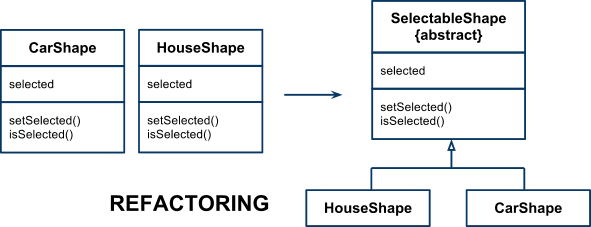
\includegraphics[scale=0.6]{images/refactor_to_template_method_pattern.png}
  \end{center}

  \begin{itemize}
    \item Refactoring adskiller sig fra design patterns idet refactoring handler om at omskrive allerede eksisterende kode, mens design patterns handler om at planlægge sit arbejde så man kan undgå at skulle benytte sig af refactoring.
  \end{itemize}

  \item Template method - en metode som flyttes fra subclasses til en superclass, og som kalder primitive operations, som kan være forskellige, i subclasses.
  \begin{itemize}
    \item Design pattern
    \item En \verb|templateMethod()| er en metode i en abstract class, som kalder abstract methods (dvs metoder som bliver defineret af subclasses som extender denne abstract class). Altså er en \verb|templateMethod()| en metode, som kalder andre metoder, som ikke endnu er blevet defineret.
    \item Eksempel: \verb|drawSelection()| i SelectableShape - \verb|drawSelection()| er defineret i SelectableShape, men kalder metoder \verb|draw()| og \verb|translate()|, som er abstract methods i SelectableShape, men som bliver defineret i CarShape og HouseShape.
  \end{itemize}

  \begin{center}
    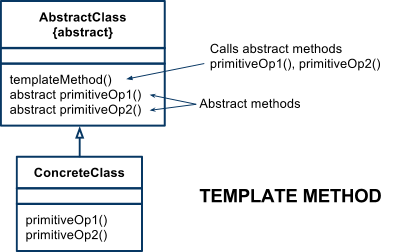
\includegraphics[scale=0.7]{images/template_method_pattern.png}
  \end{center}

\end{itemize}






\subsection{Dispositionsforslag 1}

\begin{itemize}
    \item \textbf{Interfaces}
    \begin{itemize}
        \item Hvad er et interface?
        \item Ingen instantiering, ingen implementation
        \item Eksempel: \verb|public class Hest implements Animal ...|
    \end{itemize}
    
    \item \textbf{Polymorfi og nedarvning}
    \begin{itemize}
        \item Hvad er polymorfi?
        \item Formel/aktuel type
        \item Lisskovs substitutionsprincip
        \item Eksempel: \verb|public class Manager extends Employee ...|
    \end{itemize}
    
    \item \textbf{Abstrakte klasser}
    \begin{itemize}
        \item En slags class-interface 'hybrid'
        \item Ingen instantiering, delvis implementation
        \item Eksempel: \verb|public abstract class Carnivore implements Animal ...|
    \end{itemize}
    
    \item \textbf{Template Method Pattern}
    \begin{itemize}
        \item UML-diagram
        \item Eksempel: Animal-Carnivore-Cat fra review-opgaverne
        \item Eksempel: Applets og metoderne \verb|init()|, \verb|start()|, etc.
    \end{itemize}
    
\end{itemize}

\subsection{Dispositionsforslag 2}

\begin{itemize}
    \item \textbf{Interfaces}
    \begin{itemize}
        \item Programmør behøver ikke kende egentlige klasser (jvf. Frameworks)
        \item Kan implementere mange interfaces modsat nedarvning
        \item Visibility modifiers (public, protected, private)
        \begin{itemize}
            \item private - Bruges som regel til hjælpemetoder
            \item public - Bruges til metoder der skal kunne kaldes af andre
            \item protected - Kan kun kaldes af subklasser og klassen selv
        \end{itemize}

        \item Kan ikke instantieres (kan kun bruges som statisk type)
    \end{itemize}
    
    \item \textbf{Nedarvning}
    \begin{itemize}
        \item “arve” metoder fra superklassen
        \item super keyword
        \item Kan kun nedarve fra én klasse
        \item Regler ved nedarvning
        \begin{itemize}
            \item "is-a relationen" (\textless subtype\textgreater is a \textless supertype\textgreater)
            \item Liskov substitution\footnote{Husk at Barbara Liskov er en kvinde} (en subklasse kan altid indsættes i stedet for en superklasse)
            \item Eksempel der overholder Liskov substitution
            \begin{itemize}
                \item Både is-a og Liskov glæder (Crab extends Animal (fra dIntProg) eller JonglerendeKlovn extends Klovn)
                \item Kun is-a gælder (Square extends Rectangle\footnote{Da square er mere restriktiv end rectangle})
            \end{itemize}
            
            \item Preconditions (maks lige så stærke)
            \item Postconditions (mindst lige så stærke)
        \end{itemize}
        
        \item Centralisering af kode ved at flytte det op i supertype (referer til aflevering om BankAccount)
    \end{itemize}
    
    \item \textbf{Polymorfi}
    \begin{itemize}
        \item Flere metoder med samme navn
        \begin{itemize}
            \item typesystemet sørger for korrekt kald
            \item dynamisk/statisk type
            \item Hvis man skal modellere cirkusartister har man “Linedanser” og “KanonKonge”. Programmøren ved ikke hvilken rækkefølge artisterne skal på scenen så et interface “Artist” benyttes. Interfacet har metoderne \verb udfør_nummer() og \verb buk(). Begge klasserne implementerer interfacet og programmøren kan nu håndtere forskellige artister som var de ens. Typesystemet i Java sørger for at metoden bliver kaldt på den rigtige klasse. \\
            Altså \verb artist.udfør_nummer() er forskellig alt efter om artist er af typen Linedanser eller KanonKonge. Altså metoden der bliver udført afhænger af den dynamiske type.
        \end{itemize}
        
        \item Det giver bedre muligheder for udvidelse
        \begin{itemize}
            \item Hvis der skal bruges en ny type artist kan denne blot tilføjes uden videre. Typesystemet sørger for at den korrekte metodeimplementation bliver kaldt.
        \end{itemize}
    \end{itemize}
    
    \item \textbf{TEMPLATE METHOD pattern}
    \begin{itemize}
        \item Eks. Gå over vejen (menneske og hund)
        \begin{itemize}
            \item primitive metoder (kig() og gå())
            \item Da hunden har 4 ben går den anderledes end mennesket
            \item Den kigger sig nok heller ikke så godt for
        \end{itemize}
    \end{itemize}
\end{itemize}

% DESIGN PATTERNS
\section{Design Patterns}

Design patterns er guidelines for hvordan man kan designe programmer og klasser. De kan betragtes som generelle løsninger til generelle problemer. Konceptet begrænser sig ikke til datalogi, og blev faktisk opfundet af en arkitekt. Design patterns kan sammenlignes med algoritmer som også er software mønstre, men algoritmer løser beregningsproblemer, mens design patterns løser designproblemer.

\subsection{Observer Pattern}

\begin{itemize}
  \item Hvis et objekt (Subject) starter events (som fx “mine data har ændret sig”), som andre objekter (Observers) er interesserede i at vide noget om, kan man bruge OBSERVER mønstret. Stort set alle GUI elementer (fx knapper, checkboxes, slidere) er “Subjects” i implementationer som følger OBSERVER mønstret.
  \item Subject har en samling observer objekter, som bliver tilknyttet med en attach() metode. Når en event sker, meddeler subjectet det til alle observerne.
  \item Eksempel: JButtons (Subject) har ActionListeners (Observers). Ofte bruges anonyme klasser i stedet for at lave ConreteObserver klasser:
  \begin{verbatim}
    myButton.addActionListener(new ActionListener() { 
        public void actionPerformed(ActionEvent e) {
            // do something
        }
    });
  \end{verbatim}
  
  \begin{center}
    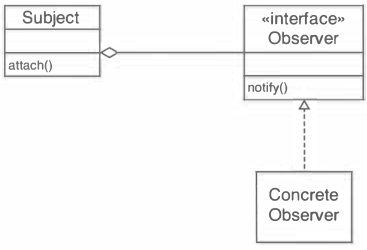
\includegraphics[scale=0.8]{images/observer_horstman.png}
  \end{center}

\end{itemize}




\subsection{Template Method Pattern}

\begin{itemize}
  \item Hvis en algoritme eller metode er brugbar i flere klasser, og kan brydes ned i “primitive operationer” (som godt kan være defineret forskelligt i de forskellige klasser) kan man bruge TEMPLATE METHOD mønstret.
  \item Metoden eller algoritmen, \verb|templateMethod()|, flyttes ind i en abstract superclass, sammen med abstract metoder for hver af de “primitive operationer”, som \verb|templateMethod()| kalder. Disse primitive operationer defineres IKKE i superclassen, men i subclasses (som extender den abstrakte superclass). 
  \item Altså er en \verb|templateMethod()| en metode som kalder andre metoder som ikke endnu er blevet defineret.
  \item Eksempel: \verb|drawSelection()| i SelectableShape - \verb|drawSelection()| er defineret i SelectableShape, men kalder metoder \verb|draw()| og \verb|translate()|, som er abstract methods i SelectableShape, men som bliver defineret i CarShape og HouseShape.
    
  \begin{center}
    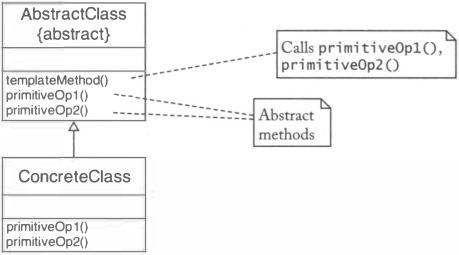
\includegraphics[scale=0.8]{images/template_method_horstman.png}
  \end{center}

\end{itemize}

\subsection{Strategy Pattern}

\begin{itemize}
  \item Hvis en klasse kan udnytte forskellige variationer af en algoritme, kan man bruge STRATEGY mønstret. LayoutManagers i Java er designet omkring STRATEGY mønstret. Containers (Context, fx JPanel, JFrame) kan udnytte forskellige layout managers (ConcreteStrategy, fx BorderLayout, GridLayout) til at arrangere deres indhold.
  \item De forskellige variationer af algoritmen defineres i klasser som implementerer et Strategy-interface. Context-klassen kalder så den rigtige metode på det konkrete Strategy-objekt. Dvs. enhver klasse som implementerer Strategy-interfacet kan benyttes af Context-klassen, men Context-klassen er også afhængig af (dependency) Strategy-interfacet.
  
  \begin{center}
    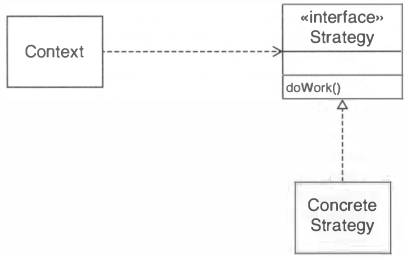
\includegraphics[scale=0.7]{images/strategy_horstman.png}
  \end{center}

\end{itemize}

\subsection{Composite Pattern}

\begin{itemize}
  \item Hvis man har behov for at kombinere en række primitive objekter i en “bundle”, som bliver opfattet af klienter som værende et enkelt primitivt objekt selv, kan man benytte COMPOSITE mønstret.
  \item Man lader en klasse (Composite) implementere det samme interface som det, de primitive objekter implementerer. Composite-klassen betragtes således af klienter på samme måde som de primitive objekter. Desuden aggregerer Composite-klassen også interfacet, hvilket betyder at den har en samling (fx ArrayList) af primitive objekter.
  \item Metoderne fra interfacet defineres i Composite-klassen ved at kalde metoderne på hvert af de primitive objekter, som er indeholdt i klassen. De skal selvfølgelig kaldes på en bestemt måde - fx skal en Bundle-klasse som indeholder Item-objekter udregne alle Item-objekternes samlede pris, når \verb|getPrice()| kaldes på Bundle.
  
  \begin{center}
    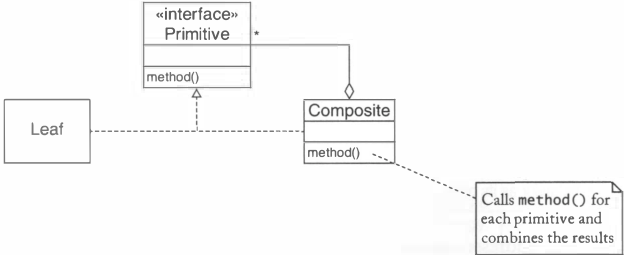
\includegraphics[scale=0.8]{images/composite_horstman.png}
  \end{center}

\end{itemize}


\subsection{Dispositionsforslag 1}

\begin{itemize}
    \item \textbf{Design Patterns}
    \begin{itemize}
        \item Hvad er design patterns?
        \item Universel kommunikation
        \item Komplet pattern: navn, kontekst, løsning og UML-diagram
    \end{itemize}
    
    \item \textbf{Observer Pattern}
    \begin{itemize}
        \item UML-diagram
        \item Subject "has-an" Observer (implementerer interfacet)
        \item Event på Subject $\rightarrow$ kald på Observer
        \item Eksempel: JButton og ActionListeners
    \end{itemize}
    
    \item \textbf{Visitor Pattern}
    \begin{itemize}
        \item UML-diagram
        \item accept(), visitNode() og visitLeaf()
        \item FileSystemNode-aflevering
        \item Sammenlign med Composite Pattern
    \end{itemize}
    
    \item \textbf{Template Method Pattern}
    \begin{itemize}
        \item UML-diagram
        \item Eksempel: Animal-Carnivore-Cat fra review-opgaverne
        \item Eksempel: Applets og metoderne \verb|init()|, \verb|start()|, etc.
    \end{itemize}
    
\end{itemize}

\subsection{Dispositionsforslag 2}

Det vigtige i dette emne er at du vælger så få at du har tid til at gå i dybden med dem alle, men ikke det er også vigtigt at du kan fylde tiden ud. Hellere have forberedt et pattern for meget end et for lidt. \\
For hvert pattern skal der være styr på UML diagrammet og hvilket problem det løser. Derudover ville det også være fint at kunne give et eksempel på brug.

\begin{itemize}
    \item \textbf{Composite}
    \begin{itemize}
        \item mønstret realiserer at en samling af objekter kan håndteres som et enkelt objekt. (Eks. en dagligvare og en indkøbspose med varer)
    \end{itemize}
    
    \item \textbf{Adapter}
    \begin{itemize}
        \item et objekt skal bruges af en klasse uden at der ændres på objektet. Objektet implementerer ikke det rigtige interface og skal adaptes til det rigtige interface.
        \item En adapter-klasse oprettes som implementerer det rigtige interface og bruger objektets metoder til at realisere de nye metoder
    \end{itemize}
    
    \item \textbf{Template Method}
    \begin{itemize}
        \item Relater til frameworks og nævn prototype pattern
        \item Hvad: en klasse der kalder primitive metoder på subklasser af et interface og kombinerer disse til en kompleks metode.
        \item Hvornår: en algoritme bruges i flere klasser. Algoritmen kan brydes ned til mindre dele. Delalgoritmerne defineres i klasserne. En superklasse kalder de primitive algoritmer i en rækkefølge så det danner den komplekse algoritme. Algoritmen er nu samlet et sted.
    \end{itemize}
    
    \item \textbf{Proxy}
    \begin{itemize}
        \item Hvad: en “stand-in” klasse for det oprindelige subjekt. Har samme metoder, dog med nogle modifikationer der gør den fordelagtig.
        \item Hvordan: en proxyklasse implementerer samme interface som det oprindelige subjekt. Proxyen kalder metoderne på subjektet.
    \end{itemize}
    
\end{itemize}

%INHERITANCE AND ABSTRACT CLASSES
\section{Inheritance \& Abstract Classes}

Nedarvning handler om at lave specialiserede udgaver af allerede eksisterende og mere generelle klasser. Eksempelvis Employee-Manager forholdet diskuteret i Horstmann kap. 6; alle Managers er Employees, men ikke alle Employees er Managers. Managers er specielle typer af Employees, som har ekstra "features".

\subsection{Superclass (generel) og subclass (specialiseret)}

\begin{itemize}
  \item "is-a" forhold: $<$subclass$>$ "is-a" $<$superclass$>$
  \begin{itemize}
    \item Java-keyword: \verb|extends|
    \item \verb|public class Manager extends Employee { ... }|
    \item En class som er erklæret \verb|final| kan ikke extendes
    \item Alle classes extender Object
  \end{itemize}

  \item Subclasses arver alle metoder og variable fra deres superclass
  \item Subclasses kan override deres superclass' metoder, dog ikke hvis de er erklæret \verb|final|
  \begin{itemize}
    \item Polymorfi bestemmer hvilken metode der kaldes vha. objektets aktuelle type. En Employee variabel kan fx indeholde et Manager objekt (Liskov's substitutionsprincip\footnote{Liskov's substitutionsprincip siger, at et object af en subclass kan benyttes nårsomhelst et objekt af dens superclass forventes. Eksempelvis kan et Manager objekt altid tildeles en Employee variabel, men ikke den anden vej rundt. Da Manager objekter altid er garanteret at have samme metoder og variable (og lidt til) som Employee objekter, er dette netop muligt.}), og polymorfien sørger for at kalde Manager-objektets overridden metode - hvis en sådan eksisterer.
    \item Override-metoder skal have samme metodesignatur (samme return type, samme parametre), som superclassen's metode.
    \item Selvom en metode er overridden kan subclasses godt kalde deres superclass' version af metoden med keywordet \verb|super|.
    \item Preconditions til overridden metoder må ikke være mere strikse end superclassens preconditions. Hvis ingen preconditions findes i superclassen må subclassens overridden metode heller ikke have preconditions.
    \item Postconditions skal omvendt være mindst ligeså strikse.
    \item En overridden metode må ikke kaste yderligere check exceptions.
  \end{itemize}

  \item Subclasses kan kun tilgå private variable gennem \verb|get()| metoder, dog kan de tilgå protected variable (en slags "intern public")
  \item Nedarvning af classes betyder, at metoder og funktionalitet er tilgængelige med det samme, og principielt behøver man ikke skrive noget yderligere kode for at bruge sin nye subclass. Implementering (\verb|implements|) af interfaces betyder derimod, at man selv skal supplere koden for hver af de metoder, som interfacet definerer.
\end{itemize}

\subsection{Abstract classes}

\begin{itemize}
  \item Abstract classes er ikke instansiérbare - dvs. man kan ikke lave objekter af abstract classes. En class tagges som abstract med keywordet \verb|abstract|.\\
  Fx: \verb|public abstract class SelectableShape implements SceneShape|
  \begin{itemize}
    \item Eksempel: SelectableShape. Abstract class der implementerer SceneShape interfacet, og som definerer nogle af interfacets metoder, men ikke alle. De metoder som ikke er definerede skal derfor defineres i subclasses (fx CarShape, HouseShape).
    \item Abstract classes implementerer typisk noget af funktionaliteten i de interfaces de evt. implementerer, men ikke alt. Resten af metoderne er abstract.
    \item Fordele: Man kan lægge al ensartet funktionalitet for flere classes i én superclass, som implementerer et interface, som er nyttigt for disse classes.
    \item Ulemper: Classes kan kun extende én superclass, men implementere adskillige interfaces.
  \end{itemize}
  
  \item Refactoring - at omskrive kode så det er "bedre" eller lettere at forstå.\\
  Fx: "Extract superclass" - Lav en superclass ud fra de fælles features to eller flere classes har.
  
  \begin{center}
    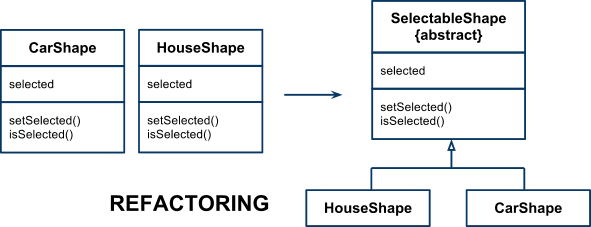
\includegraphics[scale=0.6]{images/refactor_to_template_method_pattern.png}
  \end{center}

  \begin{itemize}
    \item Refactoring adskiller sig fra design patterns idet refactoring handler om at omskrive allerede eksisterende kode, mens design patterns handler om at planlægge sit arbejde så man kan undgå at skulle benytte sig af refactoring.
  \end{itemize}

  \item Template method - en metode som flyttes fra subclasses til en superclass, og som kalder primitive operations, som kan være forskellige, i subclasses.
  \begin{itemize}
    \item Design pattern
    \item En \verb|templateMethod()| er en metode i en abstract class, som kalder abstract methods (dvs metoder som bliver defineret af subclasses som extender denne abstract class). Altså er en \verb|templateMethod()| en metode, som kalder andre metoder, som ikke endnu er blevet defineret.
    \item Eksempel: \verb|drawSelection()| i SelectableShape - \verb|drawSelection()| er defineret i SelectableShape, men kalder metoder \verb|draw()| og \verb|translate()|, som er abstract methods i SelectableShape, men som bliver defineret i CarShape og HouseShape.
  \end{itemize}

  \begin{center}
    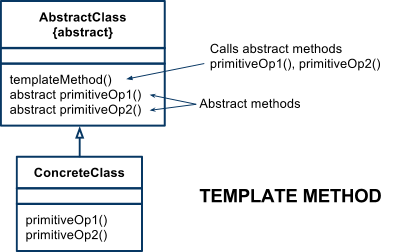
\includegraphics[scale=0.7]{images/template_method_pattern.png}
  \end{center}

  \item Protected interfaces
  \begin{itemize}
    \item protected er en mellemting mellem public og private; kan ses som "internt public" for alle subclasses til en class, men "eksternt private" for alle andre classes.
    \item Metoder kan kun bruge protected metoder/fields fra objekter af samme class som de ligger i. Fx kan HouseShape ikke kalde \verb|add()| på en CarShape, selvom de begge extender CompoundShape, som har en protected \verb|add()| metode.
    \item Protected fields bør undgås af samme grund som public fields bør undgås.
  \end{itemize}
\end{itemize}

\subsection{Hvornår er nedarvning ikke en god ide?}

\begin{itemize}
  \item Nedarvning bruges til "is-a" forhold.
  \begin{itemize}
    \item "is-a" forhold betyder at en class er en specialiseret version af en anden class. \\
Fx, "CarShape" is a "SelectableShape"
  \end{itemize}
  
  \item Aggregering bruges til "has-a" forhold.
  \begin{itemize}
    \item "has-a" forhold betyder at en class har et field hvis type er en anden class. \\
Fx, "Circle" has a "Point" - Circle classen har et Point objekt som sit centrum. Den er ikke et Point objekt i sig selv.
  \end{itemize}
  
  \item Nedarvning bør ikke bruges, hvis resultatet bryder med Liskov's substitutionsprincip.
Fx, \verb|Stack<T> extends Vector<T>| er en dum idé, da en stack og en vektor ikke har
noget med hinanden at gøre. Med en stack kan man kun push og pop elementer på
og af, og i LIFO\footnote{LIFO = Last In First Out} orden. Med en vektor kan man fjerne elementer tilfældige steder i arrayet.
\end{itemize}


\subsection{Dispositionsforslag 1}

\begin{itemize}
    \item \textbf{Nedarvning og polymorfi}
    \begin{itemize}
        \item Hvad er polymorfi?
        \item Formel/aktuel type
        \item Lisskovs substitutionsprincip
        \item Eksempel: \verb|public class Manager extends Employee ...|
    \end{itemize}
    
    \item \textbf{Abstrakte klasser}
    \begin{itemize}
        \item En slags class-interface 'hybrid'
        \item Ingen instantiering, delvis implementation
        \item Eksempel: \verb|public abstract class Carnivore implements Animal ...|
    \end{itemize}
    
    \item \textbf{Refactoring}
    \begin{itemize}
        \item Genbruge kode
        \item Fælles kode i abstrakte superklasser
        \item Mindre arbejde i underklasser
        \item Eksempel: Account-aflevering
    \end{itemize}
    
    \item \textbf{Template Method Pattern}
    \begin{itemize}
        \item UML-diagram
        \item Eksempel: Animal-Carnivore-Cat fra review-opgaverne
        \item Eksempel: Applets og metoderne \verb|init()|, \verb|start()|, etc.
    \end{itemize}
    
\end{itemize}

\subsection{Dispositionsforslag 2}

\begin{itemize}
    \item \textbf{Nedarvning}
    \begin{itemize}
        \item “arve” metoder fra superklassen
        \item visibility modifiers
        \item \textbf(super keyword)
        \item Kan kun nedarve fra én klasse
        \item Regler ved nedarvning
        \begin{itemize}
            \item "is-a relationen" (\textless subtype\textgreater is a \textless supertype\textgreater)
            \item Liskov substitution\footnote{Husk at Barbara Liskov er en kvinde} (en subklasse kan altid indsættes i stedet for en superklasse)
            \item Eksempel der overholder Liskov substitution
            \begin{itemize}
                \item Både is-a og Liskov glæder (Crab extends Animal (fra dIntProg) eller JonglerendeKlovn extends Klovn)
                \item Kun is-a gælder (Square extends Rectangle\footnote{Da square er mere restriktiv end rectangle})
            \end{itemize}
            
            \item Preconditions (maks lige så stærke)
            \item Postconditions (mindst lige så stærke)
        \end{itemize}
        
        \item Centralisering af kode ved at flytte det op i supertype (referer til aflevering om BankAccount)
    \end{itemize}
    
    \item \textbf{Polymorfi}
    \begin{itemize}
        \item Flere metoder med samme navn
        \begin{itemize}
            \item typesystemet sørger for korrekt kald
            \item dynamisk/statisk type
        \end{itemize}
        
        \item Eksempel på polymorfi
        \begin{itemize}
            \item Artist a = new Klovn();
        \end{itemize}
    \end{itemize}

    \item \textbf{Abstrakte klasser}
    \begin{itemize}
        \item Flere klasser har ens metoder
        \item Centralisering af kode
        \item tvinge subklasser til at implementere metoder
    \end{itemize}
    
    \item \textbf{TEMPLATE METHOD pattern}
    \begin{itemize}
        \item Eks. Gå over vejen (menneske og hund)
        \begin{itemize}
            \item primitive metoder (kig() og gå())
            \item Da hunden har 4 ben går den anderledes end mennesket
            \item Den kigger sig nok heller ikke så godt for
        \end{itemize}
    \end{itemize}
\end{itemize}


% EXCEPTIONS
\section{Exceptions \& Files}

Exceptions er en smart måde at håndtere programfejl på. Brug af exceptions betyder, at man kan undgå situationer hvor return-values for metodekald skal valideres på alle mulige måder, fx \verb|if (value == -1)| eller \verb|if (value != null)|. Klienter kan samtidig tvinges til at tage handling, hvis der sker fejl.

\subsection{Defensive programming}
\begin{itemize}
  \item Gå ud fra, at programmet bliver afviklet i et fjendtligt miljø med egentlige fjender, men også inkompetente brugere.
  \item Check gyldighed af inputs, return-values, etc.
\end{itemize}

\subsection{Hvis man ikke har exceptions?}
\begin{itemize}
  \item Return-values som fungerer som "fejl"-values (fx -1, null)
  \item Kræver mange if-else-statements, som gør, at det bliver mere uoverskueligt og kompliceret at separere fejlhåndteringskode fra andet kode.
  \item Ingen måde at tvinge "klienter" til at checke om returværdier er gyldige eller ej, så der er en uheldig risiko for, at programmet dermed fortsætter afvikling med ugyldige værdier, som ødelægger andre resultater - eller at programmet crasher.
\end{itemize}

\subsection{Throwable hierakiet}
\begin{itemize}
  \item Unchecked exceptions (Throwable $\leftarrow$ Exception $\leftarrow$ RuntimeException)
  \begin{itemize}
    \item Compileren kræver ikke, at unchecked exceptions håndteres, men man kan stadig håndtere dem (try-catch-blok) hvis man vil, på samme måde som med checked exceptions.
    \item Bruges til situationer hvor et program kan fejle som resultat af inkompetente programmører på den ene eller anden måde, fx hvis en metode bliver bedt om at hente data fra plads "-1" i et array. Dette er en logisk fejl, som sikkert kunne undgås vha. nogle checks.
    \item Fx NullPointerException, IllegalArgumentException
  \end{itemize}
  \item Checked exceptions (Throwable $\leftarrow$ Exception)
  \begin{itemize}
    \item Compileren kræver håndtering af checked exceptions (try-catch-blok)
    \item Bruges til situationer hvor et program kan fejle som resultat af noget, som programmøren ikke har kontrol over - fx hvis man forsøger at skrive en fil til en disk som er fuld.
    \item Fx IOException, FileNotFoundException
  \end{itemize}
\end{itemize}

\subsection{Exception handling}
\begin{itemize}
  \item For at kaste exceptions bruges \verb|throw|.
  \begin{itemize}
    \item Fx \verb|throw new IOException()|
    \item Metoder, som kaster checked exceptions skal i metode-signaturen indeholde \verb|throws| (bemærk s'et) efterfulgt af hvilke typer exceptions som kastes.
    \item Fx \verb|public void addFile(String filename) throws IOException|
    \item Metoder som kun kaster unchecked exceptions behøver ingen \verb|throws| i signaturen, men der er ingen regler imod det.
    \item Metoder kan "kaste exceptions videre" (propagate an exception). For checked exceptions skal metoderne have \verb|throws| i deres signatur, også selvom det ikke er metoden selv som kaster en exception (det kunne være et kald til en anden metode, som netop kaster exceptions).
    \item For unchecked exceptions kan \verb|throws| udelades.
  \end{itemize}
  \item Exceptions håndteres ved at "beskytte" kode, som kan kaste exceptions, med en try-blok, efterfulgt af en catch-blok, som "fanger" den type exceptions der kan blive kastet fra try-blokken.
  \begin{itemize}
    \item
      \begin{verbatim}
try {
    writeToFile(file);
} catch (IOException e) {
    System.out.println("Unable to save to " + file);
}
      \end{verbatim}
    \item Catch efterfølges af en parentes indeholdende den type af exception som der ønskes håndteret i den efterfølgende blok. Man kan have flere catch-blokke efter en try-blok, så man kan specificere hvilken type fejl programmet har lavet.
    \item \verb|catch (Exception e)| vil fange ALLE exceptions, da alle exceptions er subtyper til Exception (polymorfi).
    \item Det kræves, at en catch-blok følgende en anden catch-blok ikke fanger exceptions som er subtyper til de exceptions som fanges i ovenstående catch-blokke. Dvs. \verb|catch (Exception e)| må altså ikke komme før \verb|catch (IOException)|.
  \end{itemize}
  \item try-catch-blokke kan følges af en valgfri \verb|finally| blok.
  \begin{itemize}
    \item finally-blokken udføres uanset om der kastes en exception eller ej. Den er ofte udeladt, men kan bruges til "oprydningsarbejde".
    \item Den er ikke redundant da den også køres selvom der fx er et return-statement i try-blokken. Desuden køres den også selvom en kastet exception ikke bliver fanget af catch-blokken.
  \end{itemize}
\end{itemize}

\subsection{Error recovery and avoidance}
\begin{itemize}
  \item Man kan indkapsle try-catch-blokken i et loop, hvor man laver en slags "retry" ved at modificere elementer i catch-blokken.
  \item Fx hvis man forsøger at læse en fil som ikke eksisterer, kan man i catch-blokken ændre på filnavnet eller prøve at kigge i nærliggende mapper, inkrementere en \verb|attempts| integer \verb|MAX_ATTEMPTS| gange, og så lade try-blokken køre igen.
  \item Man kan forsøge at undgå exceptions og errors ved at lave relevante checks på return-values, før man blindt benytter dem.
  \item Typisk check \verb|if (value != null)|
\end{itemize}

\subsection{File handling}
\begin{itemize}
  \item Exceptions er meget relevante for filhåndtering, da der er mange tilfælde hvor programmøren ingen kontrol har over det miljø filerne befinder sig i.
  \begin{itemize}
    \item Typiske filhåndteringsproblemer:
    \begin{itemize}
      \item Åbne ikke-eksisterende filer.
      \item Åbne filer som er i brug.
      \item Skrive filer til en fuld harddisk.
    \end{itemize}
  \end{itemize}
  \item \verb|java.io| bibliotek til filhåndtering
  \begin{itemize}
    \item To typer filer
    \begin{itemize}
      \item Tekstfiler: filer bestående af læselige bogstaver. Håndteres med readers/writers: FileReader, BufferedReader, FileWriter
      \item Binary filer: filer bestående af byte-sekvenser. Håndteres med streams: FileInputStream, FileOutputStream
    \end{itemize}  
    \item Filen åbnes, data læses/skrives, filen lukkes.
    \begin{itemize}
      \item Til skrivning af tekstfiler benyttes FileWriter.
        \begin{verbatim}
    FileWriter writer = new FileWriter(file);
    writer.write(text);
    writer.close();
        \end{verbatim}
      \item Til læsning af tekstfiler wrappes FileReader objekter ofte i BufferedReaders, da FileReader ikke kan læse hele linjer ad gangen.
        \begin{verbatim}
    FileReader fr = new FileReader(file);
    BufferedReader reader = new BufferedReader(fr);
    reader.readLine();
    reader.close();
        \end{verbatim}
    \end{itemize}
    \item Omringes af try-catch-blok, hvori bl.a. IOExceptions fanges.
    \item Scanner
    \begin{itemize}
      \item Kan læse input fra terminalen
      \item Kan også læse input fra tekstfiler og finde betydningsfulde dele af inputtet vha. dens "parsing" metoder, fx \verb|nextInt()|.
    \end{itemize}
  \end{itemize}
  \item Serialization
  \begin{itemize}
    \item Hvis en klasse implementerer interfacet Serializable kan et objekt af klassen gemmes som en binær fil i én write operation (ObjectOutputStream)
    \item Objektet kan ligeledes indlæses igen (ObjectInputStream)
    \item Hvis dele af klassens tilstand ikke er Serializable (fx hvis man har en feltvariabel som er et HashMap) kan de markeres så de skippes af processen vha. Javas \verb|transient| keyword. Ellers kastes en exception.
  \end{itemize}
\end{itemize}


\subsection{Dispositionsforslag 1}

\begin{itemize}
    \item \textbf{Exceptions}
    \begin{itemize}
        \item Hvad er exceptions?
        \item Hvis man ikke havde exceptions?
    \end{itemize}
    
    \item \textbf{Checked vs. unchecked}
    \begin{itemize}
        \item UML-diagram, Throwable-hierarkiet
        \item Regler for checked exceptions (\verb|throws|, \verb|try-catch|)
    \end{itemize}
    
    \item \textbf{Exception handling}
    \begin{itemize}
        \item Defensive programming
        \item Exceptions kastes med \verb|throw new Exception()|
        \item Avoidance, unchecked exceptions kan ofte undgås vha. checks
        \item Recovery, for-løkke med 'attempts'-tæller for checked exceptions
    \end{itemize}
    
    \item \textbf{Filhåndtering}
    \begin{itemize}
        \item Hvorfor er exceptions relevante for filer?
        \item Tekstfiler: \verb|FileReader|, \verb|BufferedReader|, \verb|FileWriter|
        \item Andre filer: \verb|InputStream|, \verb|OutputStream|
    \end{itemize}
    
\end{itemize}

\subsection{Dispositionsforslag 2}

\begin{itemize}
    \item hvad er exceptions og hvad bruges de til
    \item hvad ville man gøre uden exceptions\footnote{I sproget C returnerer de fleste metoder en værdi der fortæller om kaldet gik godt eller skidt. For systemkald repræsenterer en negativ returværdi oftest at noget er gået galt.} (sproget C har ingen exceptions)
    \item \textbf{2 typer exceptions} (checked og unchecked)
    \begin{itemize}
        \item Tegn exceptions klassehierarki (Throwable, Exception, RuntimeException, Error)
        \item Egne exceptions (Hvilken klasse skal nedarves fra)
        \item Try / catch / finally (husk finally køres ALTID, og bruges ofte til cleanup)
        \item Throws keyword
    \end{itemize}
    
    \item \textbf{Fil håndtering}
    \begin{itemize}
        \item Meget kan gå galt
        \item Eksempler (Filen eksisterer ikke, ingen adgang til filen)
        \item Relater evt. til aflevering om filhåndtering
    \end{itemize}
    
    \item \textbf{Defensive programming}
    \begin{itemize}
        \item Minimerer antallet af fejl
        \item Tager højde for alt (især brugerinput)
        \item Brugeren er ond
        \item Programmør fejl
        \item Sørg for at programmet ikke crasher
    \end{itemize}
\end{itemize}

% THE JAVA TYPE SYSTEM AND OBJECT MODEL
\section{The Java Type System and Object Model}

\subsection{Typer og værdier}

\begin{itemize}
  \item Alle typer i Java er én af følgende:
  \begin{itemize}
    \item Primitive typer: int short long byte char float double boolean
    \item Klassetyper, fx String, Rectangle
    \item Interfacetyper, fx Comparable, Shape
    \item Arraytyper, fx String[], int[], char[]. En arraytypes elementer kaldes arrayets “component type”.
    \item Null-typen, null
  \end{itemize}

  \item Alle values i Java er én af følgende:
  \begin{itemize}
    \item En værdi til en primitiv type, fx 13, 5.0, ‘k’
    \item En reference til et objekt af en klasse, fx new String(“Hest”)
    \item En reference til et array, fx new int[] {2, 3, 5, 7, 11, 13}
    \item null
    \item Man kan ikke have værdier til interface-typer, da de ikke kan instantieres.
  \end{itemize}
\end{itemize}

\subsection{Subtype-forhold}

\begin{itemize}
  \item Subtype-forholdet i Java følger Liskov’s substitutionsprincip om, at subtyper kan benyttes hvor supertyper forventes. Vi betragter to typer, S og T. S er en subtype til typen T, hvis én af følgende regler passer:
  \begin{itemize}
    \item S og T er samme type
    \item S og T er begge klassetyper, og S er en direkte eller indirekte subclass til T
    \item S og T er begge interface-typer, og S er direkte eller indirekte subinterface til T
    \item S er en klassetype, T er en interface-type, og S eller en superclass til S implementerer T eller et subinterface til T
    \item S og T er arraytyper, og component-typen til S er en subtype til component-typen til T
    \item S er ikke en primitiv type, og T er Object
    \item S er en arraytype, og T er Cloneable eller Serializable
    \item S er null og T er ikke en primitiv type
  \end{itemize}

  \item Ved subtype-forhold mellem to arraytyper kan man “trække array brackets fra” begge arrays indtil én eller begge typer ingen brackets har.
  \begin{itemize}
    \item \verb|Object[]| og \verb|int[]|, træk brackets fra på begge arrays, \verb|Object| og \verb|int|, og da \verb|int| er en primitiv type er den ikke en subtype til \verb|Object|, og dermed er \verb|int[]| ikke en subtype til \verb|Object[]| og omvendt. \verb|int[]| er dog en subtype til \verb|Object|, så \verb|int[][]| er en subtype til \verb|Object[]|.
  \end{itemize}
  
  \item Compiler checker kun formelle typer, hvilket vil sige, at selv om man fodrer en subtype til en supertype (Manager i Employee variabel, Liskov substitution), kan man kun kalde supertypens metoder, fordi compileren altid kun kigger på formelle typer.
  \begin{itemize}
    \item Typecasting betyder at man omdanner et objekts statiske/formelle type til en anden type, fx
    \begin{verbatim}
      Employee e = new Manager();
	  e.getBonus()	              // COMPILE ERROR!
	  ((Manager)e).getBonus()     // OK!
    \end{verbatim}
    \item Primitive typer kan også typecastes, men der er nogle bestemte termer i den forbindelse:
    \begin{itemize}
      \item Widening, når man fx caster en int til en double. (\verb|2 -> 2.0|)
    Sker automatisk! Fx double \verb|x = 2 -> x = 2.0|
      \item Narrowing, når man fx caster en double til en int. (\verb|2.5 -> 2|)
    Kræver typecast! Fx \verb|int y = (int) 5.2 -> y = 5|
    \end{itemize}
  \end{itemize}
\end{itemize}

\subsection{Wrappers (aka. Snoop Dogg)}

\begin{itemize}
  \item De 8 primitive typer har tilhørende wrappers (klassetyper): Integer, Short, Long, Byte, Character, Float, Double, Boolean. De har altså samme navne som deres primitive modstykker, pånær Integer (int) og Character (char).
  \item Wrapper-classes kan wrappe primitive typer i objekter, hvor det er nødvendigt. Fx hvis man skal have en ArrayList med ints. ArrayList kan ikke have primitive typer.
  \item Auto-boxing er den automatiske konvertering mellem primitive typer og wrapper objekter. Dette gør at man ganske enkelt kan tilføje int-værdier til ArrayLists af Integers, uden at skulle konvertere manuelt først.
\end{itemize}

\subsection{Enum}

\begin{itemize}
  \item Enumerated types er typer med et endeligt sæt værdier. Eksempler på enum typer er Suit med fire værdier: SPADE, CLUB, HEART, DIAMOND, eller Size, som fx kunne have værdierne: SMALL, MEDIUM, LARGE.
  \item Keywordet enum definerer en class med en private constructor (nye objekter kan ikke laves fra den) med nogle fields tagged som \verb|public static final|. Det er forsvarligt at lade dem være public, idét klassen ingen metoder har, og dens fields er alle final.
\end{itemize}

\subsection{Type inquiry}

\begin{itemize}
  \item Man kan teste om et objekt eller en expression er en reference til et objekt af en bestemt type, eller én af dens subtyper med instanceof operatoren.
  \begin{itemize}
    \item \verb|if (e instanceof Shape)|
  \end{itemize}

  \item Man kan finde et objekts klasse med getClass() metoden. Den returnerer et Class objekt. Dette objekt indeholder en masse information om det objekt, metoden blev kaldt på. Fx navnet på den klasse objektet tilhører, eller klassens eventuelle superclass.
  \begin{itemize}
    \item Med getName() kaldt på et Class objekt kan man få det præcise klassenavn for et objekt.
    \item Class objekter kan beskrive enhver type, også primitive typer.
  \end{itemize}

  \item Vil man teste om et objekt tilhører en bestemt class, kan man kalde \verb|getClass()| på objektet og sammenligne med den bestemte class således:
  \begin{itemize}
    \item \verb|if (e.getClass() == Rectangle.class)|
  \end{itemize}

  \item Type inquiry bør ikke bruges som en erstatning for polymorfi.
\end{itemize}

\subsection{The Object class - mother of all classes}

\begin{itemize}
  \item Alle Java-classes er subclasses til Object. Hvis en class ikke extender nogle andre classes er den en direkte subclass til Object. Derfor er alle metoder i Object tilgængelige for alle objekter. De fire vigtigste (som også altid bør overrides i custom classes) er:
  \begin{itemize}
    \item toString() som returnerer en String-repræsentation af objektet.
    \begin{itemize}
      \item Bruges automatisk af forskellige standard-metoder. Fx hvis man prøver at printe et objekt vha. \verb|System.out.println()|.
    \end{itemize}
    
    \item equals() som sammenligner et objekt med et andet.
    \begin{itemize}
      \item Man kan nemt sammenligne to ints med hinanden som (\verb|x == y|), men bruger man == operatoren på objekter sammenlignes objekternes referencer.
      \item Det ønskes ofte at to objekter betragtes som værende “ens”, hvis dele eller hele tilstande af objekter er ens. Fx kan to Beer-objekter betragtes som ens hvis deres name og percent fields er ens. \\
    Hvis to lister indeholder de samme elementer i forskellige rækkefølger 	kan de også i nogle situationer betragtes som ens.
      \item Den perfekte equals metode starter ifølge Horstmann således:
      \begin{verbatim}
        if (this == otherObject) return true;
	    if (otherObject == null) return false;
	    if (getClass() != otherObject.getClass()) return false;
      \end{verbatim}
      \item Metoden skal være reflexive (\verb|x.equals(x)|) og symmetrisk (\verb|x.equals(y)   <->   y.equals(x)|)
    \end{itemize}
    
    \item hashCode() som returnerer en hash code for objektet.
    \begin{itemize}
      \item Hash codes skal være konsistente med equals metoden, så to objekter som “equals” hinanden genererer samme hash codes.
    \end{itemize}
    
    \item clone() som returnerer en kopi/klon af objektet.
    \begin{itemize}
      \item Cloneable interface skal implementeres
      \item Der skælnes mellem deep og shallow copies af objekter vha. clone metoden.
      \item En shallow copy er en kopi, som ganske enkelt bare kopierer alle værdierne i originalens fields (\verb|orig.x = ? -> clone.x = orig.x|). Hvis disse værdier er objektreferencer (hvilket de er, hvis de ikke er primitive værdier), vil kopien nu dele objektreferencer med originalen, hvilket betyder at en ændren i kopiens værdier også ændrer på originalens værdier!
      \item En deep copy er en kopi som er magen til originalen, men har sine egne field-værdier (\verb|orig.x = ? -> clone.x = new x|). Ændringer i kopien ændrer således ikke på originalen.
      \item En “sufficiently deep copy” er en kopi som kun opretter nye objektreferencer til objekter som er mutérbare. String er immutérbare, så typiske name fields er ikke kritiske.
    \end{itemize}
  \end{itemize}
\end{itemize}

\subsection{Serialization}

\begin{itemize}
  \item Man kan gemme objekter som binære filer, hvis klassen objekterne tilhører implementerer \verb|Serializable| interfacet.
\end{itemize}

\subsection{Generic Types}

\begin{itemize}
  \item Generics er typer som har en eller flere type-variable, som betegnes med bogstavet E, fx \verb|ArrayList<E>| som altså instantieres med en ikke-primitiv type. Det kunne være \verb|ArrayList<Integer>| eller \verb|ArrayList<String>|. Metoderne i generic types arbejder med dette E, som altså ved instantiering er en egentlig type.
\end{itemize}



\subsection{Dispositionsforslag 1}

\begin{itemize}
    \item \textbf{Typer}
    \begin{itemize}
        \item Hvad er typer? Hvilke findes der?
        \item Primitive typer, reference-typer
        \item \verb|null|-pointers
    \end{itemize}
    
    \item \textbf{Subtype-forhold}
    \begin{itemize}
        \item Keywords: \verb|extends| og \verb|implements|
        \item Casting af reference-typer
        \item Casting af primitive typer, widening/narrowing
    \end{itemize}
    
    \item \textbf{Generics og Wrappers}
    \begin{itemize}
        \item Generics omgår IntArrayList, StringArrayList, etc.
        \item Tillader at benytte en generisk klasse med vilkårlige typer
        \item Wrapper-klasser nødvendige for primitive typer
    \end{itemize}
    
    \item \textbf{The Object Class}
    \begin{itemize}
        \item Metoder: \verb|toString()|, \verb|equals()|, \verb|hashCode()|
        \item Forhold mellem \verb|equals()| og \verb|hashCode()|
        \item Evt. \verb|clone()|
    \end{itemize}
    
    \item \textbf{Cloning}
    \begin{itemize}
        \item Deep vs. shallow
        \item Java API'en, ArrayList
        \item Pointer-diagram
    \end{itemize}
    
\end{itemize}

\subsection{Dispositionsforslag 2}

\begin{itemize}
    \item \textbf{Typer}
    \begin{itemize}
        \item Primitive typer
        \begin{itemize}
            \item wrappers og auto boxing
            \item widening / narrowing
            \item type casts
        \end{itemize}
        
        \item Reference typer
        \begin{itemize}
            \item klasse / interface / array
            \item statisk / dynamisk type (skriv kode og forklar)
        \end{itemize}
        
        \item null (special case da null ikke er en type)
    \end{itemize}
    
    \item \textbf{Object klassen}
    \begin{itemize}
        \item Alle referencetyper nedarver fra Object
        \item Implementerer generelle metoder
        \item \textbf{Equals} (overvej at skrive kode\footnote{Det tager lang tid at skrive koden og det er vigtigt at det er helt korrekt. Overvej om det er det værd, eller om du hellere vil have mere tid til at tale om de andre emner.})
        \begin{itemize}
            \item $x=x$
            \item $x=y \implies y=x$
            \item $x=y \and y=z \implies x=z$
        \end{itemize}
        
        \item \textbf{Clone} (deep og shallow) - overvej at komme ind på immutable klasser
    \end{itemize}
    
    \item \textbf{Generics}
    \begin{itemize}
        \item Wildcards / extends / super
        \item Eksempel på brug \verb Collections.sort()
        \item Kodeeksempel på generisk klasse
    \end{itemize}
\end{itemize}

% FRAMEWORKS
\section{Frameworks \& Collections}

Frameworks er en samling af klasser som alle arbejder sammen og er relevante for et bestemt emne. Fx er Swing et framework, og dets klasser benyttes alle til at lave GUI’er med. Et andet framework er Applet, som bruges til at lave Java applets med, så de kan køres i web browsers.


\subsection{Frameworks og libraries}

\begin{itemize}
  \item Frameworks adskiller sig fra normale program libraries på forskellige måder
  \begin{itemize}
    \item Inversion of control - I modsætning til almindelige libraries fungerer det meste af execution flowet for et framework i selve framework klasserne. Dvs. frameworkets metoder kan overrides, men det er frameworket som sørger for at kalde dem. Dette fænomen kaldes også Hollywood-princippet: “Don’t call us, we call you.”
    \item Extensibility - Brugere kan benytte frameworkets default behaviour eller override og specialisere dets metoder.
    \item Niks pille - Frameworkets kode må generelt ikke ændres. Brugere er nødt til at extende og override for at specialisere funktionalitet.
  \end{itemize}

  \item Frameworks er ikke design patterns, og der er ingen egentlige design regler for hvordan frameworks skal se ud - de består udelukkende af et sæt klasser, som udgør en slags generel service for en bestemt type program, og de benytter typisk mange forskellige design patterns.
\end{itemize}

\subsection{Applets}

\begin{itemize}
  \item Applets er programmer som afvikles i web browsers. java.applet er et framework, som bruges til lige netop det formål.
  \item I de fleste selvstændige programmer er der en main metode, som er det første der bliver kørt når programmet starter. I Applet-frameworket er denne metode allerede defineret, og programmer som extender Applet, skal bare override nogle eller alle af følgende metoder:
  \begin{itemize}
    \item init - Kaldes én gang, lige når appletten loades.
    \item start - Kaldes når appletten startes (efter init)
    \item stop - Kaldes når appletten eller browseren lukkes
    \item destroy - Kaldes når browseren lukkes for at frigive resourcer
    \item paint - Kaldes når appletten skal repaintes (ofte).
  \end{itemize}

  \item Framework karakteristika for applets:
  \begin{itemize}
    \item Applet-programmøren extender Applet frameworket (inheritance)
    \item Applet-klassen sørger for alle de trivielle ting, som at parse parametre og checke hvornår appletten er synlig og sådan. Applet-programmøren overrider bare metoder som ønskes specialiseret.
    \item Inversion of control gør, at programmøren ikke bekymres med hvornår og hvordan metoderne skal afvikles. Det sørger frameworket for.
  \end{itemize}
\end{itemize}

\subsection{Collections}

\begin{itemize}
  \item Collections er både en samling af almene datastrukturer og et framework for nye collection klasser. Frameworket indeholder nogle forskellige interfaces, fx:
  \begin{itemize}
    \item \textbf{Collection} - Det mest generelle collection interface
    \item \textbf{Set} - En usorteret collection some ikke tillader duplicates
    \item \textbf{SortedSet} - En sorteret collection som ikke tillader duplicates. Elementerne sorteres vha. Comparable eller Comparator
    \item \textbf{List} - En ordnet collection der kan indeholde duplikater
  \end{itemize}

  \item Frameworket tilbyder desuden konkrete klasser som implementerer disse interfaces. Nogle af de vigtigste er:
  \begin{itemize}
    \item \textbf{HashSet} - Et set som bruger hashing/hash codes til at finde dets elementer
    \item \textbf{ArrayList} - En liste som internt er baseret på arrays. ArrayLists er gode, hvis man ønsker hurtig “random access” i listen, da dens “lookups” fungerer som i arrays. Til gengæld er ArrayList langsom til at tilføje og fjerne elementer, da der ved disse operationer laves en kopi af det nuværende array, plus/minus ét element.
    \item \textbf{LinkedList} - En liste som ikke er baseret på arrays. LinkedLists er gode hvis man ønsker hurtige add/remove metoder, men deres “lookups” er meget langsomme sammenlignet med ArrayLists, da LinkedLists altid gennemløbes fra start til det index man søger.
  \end{itemize}

  \item AbstractCollection er en abstrakt klasse, som implementerer Collection interfacet, og definerer alle metoderne, undtagen \verb iterator() og \verb size(). Metoder som \verb toArray() bruger netop \verb iterator() og \verb size(), hvilket vidner om Template Method designmønstret.
  \begin{itemize}
    \item AbstractCollection efterlader kun følgende to metoder til subclasses:
    \begin{itemize}
      \item \verb|int size()|
      \item \verb|Iterator<E> iterator()|
    \end{itemize}
    
    \item De fleste konkrete collection classes som extender AbstractCollection overrider dog \verb add() metoden, da AbstractCollection’s version er en dummy udgave som bare kaster en UnsupportedOperationException, hvilket giver mening for collections som skal være immutable.
  \end{itemize}
\end{itemize}


\subsection{Dispositionsforslag 1}

\begin{itemize}
    \item \textbf{Frameworks}
    \begin{itemize}
        \item Frameworks vs. libraries
        \item Inversion of Control
        \item java.lang.Math er et library, ingen IoC
        \item Java Applets hører til et framework
    \end{itemize}
    
    \item \textbf{Applets}
    \begin{itemize}
        \item Simpelt framework
        \item Metoderne \verb|init()|, \verb|start()|, etc. $\rightarrow$ IoC
    \end{itemize}
    
    \item \textbf{Collections}
    \begin{itemize}
        \item Alle niveauer af et framework
        \item Interfaces, fx List
        \item Abstrakte klasser, fx AbstractCollection
        \item Færdige klasser, fx ArrayList
        \item Sammenligning af forskellige collections, ArrayList vs TreeSet
    \end{itemize}
    
    \item \textbf{Template Method Pattern}
    \begin{itemize}
        \item UML-diagram
        \item MultiSet-aflevering
    \end{itemize}
    
\end{itemize}

\subsection{Dispositionsforslag 2}

\begin{itemize}
    \item \textbf{Framework vs program library}
    \begin{itemize}
        \item Hollywood princippet “Don’t call us, we call you”
        \item hot spots / frozen spots
        \item Eks. RPG spil eller applets\footnote{Det vigtige her er at du har styr på dit eksempel og føler dig sikker på at tale om det.}
        \begin{itemize}
            \item Extend applet med metoderne (init(), start(), stop() og paint()) frameworket kalder selv disse metoder. Appletklassen er altså et hot spot.
        \end{itemize}
    \end{itemize}
    
    \item \textbf{Prototyper (PROTOTYPE pattern)}
    \begin{itemize}
        \item Frameworket skal kunne kalde brugerens klasser
        \item Laver nye objekter ved at klone en prototype
    \end{itemize}
    
    \item \textbf{Collections framework}
    \begin{itemize}
        \item sort / shuffle / min / max
        \item Collection interface (hot spot) (generisk)
        \begin{itemize}
            \item set (ingen dupletter) vs. list (elementers rækkefølge er bibeholdt)
            \item Benyt muligvis muligheden for at tale om generiske klasser
        \end{itemize}

        \item AbstractCollection\textless E\textgreater
        \begin{itemize}
            \item Opret nye collections ud fra denne klasse der implementerer de fleste metoder
            \item \textbf{TEMPLATE METHOD pattern} (vær klar på at give specifikt ekesmpel)
        \end{itemize}
    \end{itemize}
\end{itemize}














% MULTITHREADING

\section{Multithreading}


Tråde er er programstykker som kan eksekveres parallelt med hinanden, dvs. "på samme tid". På single-core systemer skifter operativsystemet konstant mellem trådene, hvilket giver illusionen af, at de kører parallelt. På multi-core systemer kan operativsystemet derimod virkelig afvikle tråde parallelt - én på hver core.

\subsection{Fordele}

\begin{itemize}
  \item Gør det muligt at separere program-kode fra kontrol-kode, fx kan lange rekursive beregninger udføres i én tråd, mens main-tråden fortsat reagerer på inputs fra brugeren.
  \item Kan således forhindre at programmer "fryser" mens lange beregninger finder sted.
\end{itemize}

\subsection{Ulemper}

\begin{itemize}
  \item Der kan opstå problemer, fx race conditions ved synkronisering hvis flere tråde deler data.
  \item Deadlocks hvis alle aktive tråde venter på at nogle andre tråde "gør noget"
\end{itemize}

\subsection{Runnable interfacet}

\begin{itemize}
  \item En class som implementerer Runnable interfacet skal override metoden run(), hvorefter et Thread-objekt kan laves med et objekt af denne "Runnable class". Herefter kaldes start() på Thread-objektet, og så afvikles koden i Runnable objektets run() metode.
  \begin{verbatim}
    Runnable r = new MyRunnable();
    Thread t = new Thread(r);
    t.start();
  \end{verbatim}
  \item UML diagram
  
  \begin{center}
    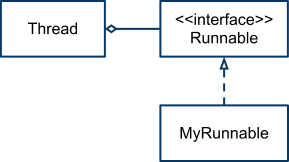
\includegraphics[scale=0.6]{images/runnable_uml.png}
  \end{center}
    
\end{itemize}

\subsection{Selfishness}

\begin{itemize}
  \item En tråd skal lade andre tråde "komme til", ellers er den selfish. På nogle platforme kan en selfish tråd forhindre andre tråde i at blive afviklet, hvilket ødelægger formålet med tråde.
  \item Tråde kan sættes til at "sove" med sleep(). Når en tråd sættes til at sove betyder det, at andre tråde kan komme til.
  \item En tråds afviklingstid kaldes en "time slice".
  \begin{itemize}
    \item main() metoden i ethvert Java program er sin egen tråd.
    \item Hvis man har startet flere tråde i sit program afsluttes det først når alle trådene er færdige, eller er blevet interrupted.
  \end{itemize}
\end{itemize}

\subsection{Tilstand}

\begin{itemize}
  \item Diagram
  
  \begin{center}
    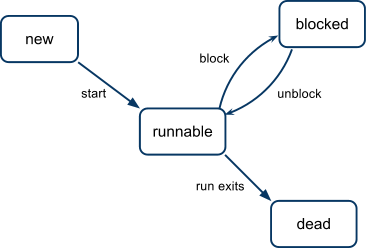
\includegraphics[scale=0.7]{images/thread_states.png}
  \end{center}
    
  \begin{itemize}
    \item Når der laves et nyt Thread objekt er den new. Når \verb start() metoden kaldes bliver tråden runnable. Herfra er tråden klar til at blive kørt. Tråden kan blive blocked hvis der kaldes \verb wait() eller \verb sleep(). Dette sker som regel når tråden venter på en lås. Når tråden vækkes af enten \verb notify() eller \verb signal() bliver den igen runnable. Når \verb run() metoden returnerer dør tråden.
  \end{itemize}

  \item En tråd kan være blocked hvis den sover, venter på input/output, venter på en lock eller en condition.
  \item Når en tråd er blocked forbliver den blocked indtil den event den venter på sker. Fx, hvis en tråd sover bliver den først runnable igen når dens sovetid er gået.
\end{itemize}

\subsection{interrupt()}

\begin{itemize}
  \item Tråde kan afbrydes/stoppes med \verb|interrupt()| 
  \item sleep() og wait() kaster en InterruptedException, hvis interupt() kaldes på en "sovende tråd". Denne exception skal fanges, og man bør derfor omringe al koden i run() med en try-blok.
  \item Hvis tråden ikke er blocked vil interrupt() bare sætte trådens interrupted field til true. Dette field kan checkes med metoden isInterrupted().
  \item I tilfælde af I/O eller andet "beskidt" arbejde bør tråde altid have noget oprydningskode efter try-blokken.
\end{itemize}

\subsection{Race conditions}

\begin{itemize}
  \item Når flere tråde deler data, som kan korrupteres hvis trådene ikke afvikles i en bestemt rækkefølge.
  \item Hvis to tråde fx forsøger at lægge nyt indhold i en queue, og samtidig inkrementerer queuens tail, så kan race conditions gøre, at en tråd ikke når at inkrementere tailen før en ny tråd tager over. I så fald overskrives den første tråds data. Se evt. Horstmann s. 376
  \item Locks kan bruges til at blokkere alle andre tråde, som forsøger at tilgå den samme data som den nuværende tråd, indtil denne er færdig med sin kode. Når den første tråd frigiver locken, bliver de andre tråde unblocked.
  \begin{itemize}
    \item En tråd kan "acquire" en lock ved at kalde lock() på locken. Hvis en anden tråd forsøger at acquire en locked lock bliver den blocked, indtil den første tråd kalder unlock() på locken.
    \item Locks sikrer, at en tråd færdiggør sit arbejde med noget data før eventuelle andre tråde kan korruptere det.
  \end{itemize}

  \item Deadlocks - når ingen tråde kan fortsætte fordi de venter på at en anden tråd gør noget først. Fx hvis en tråd venter på at der bliver plads i en fuld queue, men queuen ikke bliver tømt, da ingen tråde kan få locken, så de kan fjerne elementer fra queuen.
  \begin{itemize}
    \item En lock kan have et tilknyttet Condition objekt. Hvis man kalder await() på et Condition objekt kan man lade andre tråde få den lock som den nuværende tråd har.
    \item En tråd, som har kaldt await() på et tilhørende Condition objekt er blokkeret indtil en anden tråd kalder signalAll() på Condition objektet som tråden venter på.
    \item Typisk laves checks på Condition objekter i while-løkker, \\
    fx \verb|while (not OK to proceed) Condition.await()|
  \end{itemize}

  \item Der er object locks bygget ind i alle Java objekter. Disse kan bruges på samme måde som ReentrantLocks, men i stedet for at opsætte locks skal synkroniserede metoder tagges med "synchronized" keywordet, fx "\verb|public synchronized void add(E newValue)|".
  \begin{itemize}
    \item Når en synchronized metode kaldes låses object locken.
    \item Når en synchronized metode er færdig frigives object locken.
    \item Object locks har én (anonym) Condition.
    \item \verb|wait() <-> await()| og \verb|notifyAll() <-> signalAll()|, dvs. man kan frigive object locken på næsten samme måde som med ReentrantLock, og ligeledes signalere til alle ventende tråde.
  \end{itemize}

  \item java.util.concurrent biblioteket har en BlockingQueue klasse, som er designet med race conditions i baghovedet. Queuens put() og take() metoder afventer på hhv. plads i køen og elementer i køen, før de fortsætter.
  \begin{itemize}
    \item Concurrent = samtidig
  \end{itemize}

\end{itemize}



\subsection{Dispositionsforslag 1}

\begin{itemize}
    \item \textbf{Tråde}
    \begin{itemize}
        \item Hvad er tråde? Hvad bruges de til?
        \item Tråde i Java; \verb|implements Runnable| eller \verb|extends Thread|
        \item UML diagram (Horstmann s. 364)
    \end{itemize}
    
    \item \textbf{Tilstande}
    \begin{itemize}
        \item new, runnable, blocked, dead
        \item interrupt()
    \end{itemize}

    \item \textbf{Race conditions}
    \begin{itemize}
        \item Deadlocks (og livelocks)
        \item Queue eksempel; korruptering af data, tegn på tavlen
        \item ReentrantLocks vs. object locks
        \item \verb|wait()| og \verb|notify()|
    \end{itemize}

    \item \textbf{java.util.concurrent og BlockingQueue}
    \begin{itemize}
        \item Masser af færdige, brugbare klasser
        \item Metoder som \verb|take()| blocker automatisk
    \end{itemize}
\end{itemize}

\subsection{Dispositionsforslag 2}

\begin{itemize}
    \item \textbf{Tråde}
    \begin{itemize}
        \item Hvad er en Tråd
        \begin{itemize}
            \item Producer / Consumer\footnote{En producer tråd laver data, fx læser ord i en fil. Oftest tilføjes denne data til en kø. Consumer tråd bruger denne data, fx lægger antal ord sammen for flere filer. Normalvis venter consumertråden på at der kommer data i køen.}
        \end{itemize}
        
        \item Hvorfor bruge threads
        \begin{itemize}
            \item Referer til binomial aflevering, hvor beregningen kunne køres i en separat tråd, så GUIen ikke ville fryse
            \item Kan benytte alle processorens kerner
        \end{itemize}
        
        \item \textbf{Runnable} - Hvordan laves en tråd
        \begin{itemize}
            \item Implementer Runnable interfacet og benyt start() metoden på Thread
            \item 4 states (new, runnable, blocked, dead) - lav tegning
        \end{itemize}
        
        \item Interrupts - try/catch i run() metoden
    \end{itemize}
    
    \item \textbf{Synkronisering}
    \begin{itemize}
        \item \textbf{Race conditions}
        \item \textbf{Locking}
        \begin{itemize}
            \item Eksplicitte locks fra java.util.concurrency (\verb|await()| / \verb|signalAll()|)
            \item Synchronized keyword (Nemmere at bruge, men mindre fleksible)
            \item \textbf{Deadlocks og livelocks\footnote{Livelocks er ikke ligeså vigtive som deadlocks, så undlad at snakke om disse hvis du ikke har styr på dem.}}
        \end{itemize}
        
        \item Køer
        \begin{itemize}
            \item Udveksling af data mellem tråde
            \item Benyttes ofte i forbindesle med producer/consumer
            \item Undgå raceconditions ved at benytte en synkroniseret kø fx LinkedBlockingQueue
        \end{itemize}
    \end{itemize}
\end{itemize}



% Necessary for correct page numbering
% http://tex.stackexchange.com/a/116014
% Note: This increases compilation time!
\phantom{\cite{?}}

\end{document}